\documentclass[../sparc.tex]{subfiles}
\graphicspath{{\subfix{../images/}}}
\begin{document}

%%%%%%%%%%%%%%%%%%%%%%%%%%%%%%%%%%%%%%%%%%%%%%%%%%%%%%%%%%%%%%%%%%%%%%%%%%%%%%%%
\section{Аналогово-цифровое преобразование}
\newglossaryentry{АЦП}{name=АЦП, description={Аналогово-Цифровой Преобразователь}}
\newglossaryentry{ЦАП}{name=ЦАП, description={Цифро-Аналоговый Преобразователь}}
\newglossaryentry{ADC}{
  name=ADC,
  description={Analog-to-Digital Converter (см. \gls{АЦП})}}
\newglossaryentry{DAC}{
  name=DAC,
  description={Digital-to-Analog Converter (см. \gls{ЦАП})}}


Мы могли заметить в главе \ref{section:analog-ports}, что при считывании с
аналогового порта получается значения в диапазоне от 0 до 1023.  Число 1023
подозрительно похоже на число 1024, которое в программировании встречается
достаточно часто -- не удивительно, ведь 1024 это степень двойки ($2^{10}$).

Давайте разберёмся, почему же значения с аналогового порта в Arduino находятся
именно в таком диапазоне.  Начнём с того, что аналоговый порт каким-то образом
преобразует входящий аналоговый сигнал в цифровое (двоичное) представление,
которое мы и видим в программе.

Операцию преобразования аналогового сигнала в цифровой выполняет компонент,
называемый \emph{Аналого-Цифровой Преобразователь} (сокращённо \gls{АЦП}.)  В
роли АЦП может выступать как отдельная микросхема, так и сам микроконтроллер.
Схематически аналогово-цифровой преобразователь можно изобразить, как показано
на рис. \ref{fig:adc-schematics}.

По-английски ``АЦП'' -- ``Analog-to-Digital Converter'' (сокращённо \gls{ADC}.)

\begin{figure}[ht]
  \centering
  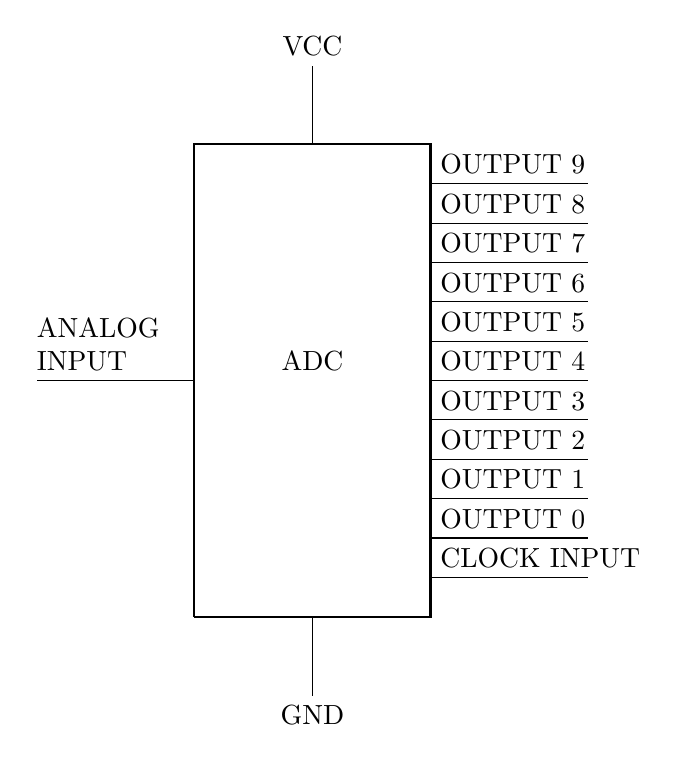
\begin{tikzpicture}
    \draw[thick] (0, 0) -- (0, 6.0) -- (3, 6.0) -- (3, 0) -- (0, 0);
    \draw (1.5, 3.00) node[right, above] {ADC};
    \draw (3, 0.5) node[anchor=south west] {CLOCK INPUT} -- (5, 0.5);
    \foreach \n/\y in {0/1.0, 1/1.5, 2/2.0, 3/2.5, 4/3.0, 5/3.5, 6/4.0, 7/4.5, 8/5.0, 9/5.5} {
      \draw (3, \y) node[anchor=south west] {OUTPUT \n} -- (5, \y);
    };
    \draw (0, 3.00)
    -- (-1, 3.00) node[left, above, text width=2cm] {ANALOG INPUT}
    -- (-2, 3.00);
    \draw (1.5, 6.0) -- (1.5, 7.0) node[right, above] {VCC};
    \draw (1.5, 0) -- (1.5, -1) node[right, below] {GND};
  \end{tikzpicture}
  \caption{Схематическое изображение 10-битного аналогово-цифрового
    преобразователя.}
  \label{fig:adc-schematics}
\end{figure}

На вход АЦП (``ANALOG INPUT'') подаётся аналоговый сигнал, а на выходах
(``OUTPUT 0'' .. ``OUTPUT 9'') кодируется значение входного сигнала в каждый
момент времени в виде набора логических уровней ``HIGH'' (``1'') / ``LOW''
(``0''.)  Самому АЦП требуется также питание -- для этого как раз предназначены
выводы ``VCC'' и ``GND''.

\example { На вход АЦП подаётся 2.5В.  На выходах формируется двоичное значение
  ``1000000000'', что соответствует числу $2^9 = 512$, которое может быть
  получено в программе микроконтроллера. }

Преобразование аналогового сигнала в цифровой внутри АЦП проходит в три этапа:
\begin{enumerate}

\item \textbf{Дискретизация.} Выбираются значения из исходного аналогового сигнала через
  равные временные промежутки (\ref{fig:discretization}.)

  \begin{figure}[h]
    \centering
    \begin{tikzpicture}
      [
        declare function={
          f(\x)=2 + exp(-\x/10)*( cos(deg(\x)) + sin(deg(\x))/10 ) * 2;
        }
      ]

      \begin{axis}[
          width = \textwidth,
	        xmin = 0, xmax = 30,
	        ymin = 0, ymax = 5.0,
          xlabel={$t$},
          ylabel={$U$}
        ]

	      \addplot[
		      domain = 0:30,
		      samples = 200,
		      smooth,
		      thick,
		      blue,
	      ] {
          2 + exp(-x/10)*( cos(deg(x)) + sin(deg(x))/10 ) * 2
        };

        \foreach \x [evaluate={\y=f(\x)}] in {1, 2, ..., 30} {
          \addplot[red]
          coordinates {
            (\x, 0) (\x, \y)
          };
          \addplot[red, mark = *, mark size=1.0pt]
          coordinates { (\x, \y) };
        };

        \legend{
	        Аналоговый сигнал,
          Замеры значения
        }
	    \end{axis};
    \end{tikzpicture}
    \caption{Дискретизация.}
    \label{fig:discretization}
  \end{figure}

  Характеристика, отражающая эти временные промежутки, называется \emph{частотой
  дискретизации}.

  \begin{figure}[h]
    \centering
    \begin{tikzpicture}
      [
        declare function={
          f(\x)=2 + exp(-\x/10)*( cos(deg(\x)) + sin(deg(\x))/10 ) * 2;
        }
      ]

      \begin{axis}[
          width = \textwidth,
	        xmin = 0, xmax = 30,
	        ymin = 0, ymax = 5.0,
          xlabel={$t$},
          ylabel={$U$},
        ]

	      \addplot[
		      domain = 0:30,
		      samples = 200,
		      smooth,
		      thick,
		      cyan
	      ] {
          2 + exp(-x/10)*( cos(deg(x)) + sin(deg(x))/10 ) * 2
        };

        \foreach \x [evaluate={\y=f(\x); \xnext=\x + 1; \ynext=f(\x + 1)}] in {1, 2, ..., 30} {
          \addplot[red]
          coordinates {
            (\x, \y) (\xnext, \y) (\xnext, \ynext)
          };
          \addplot[red, mark = *, mark size=1.0pt]
          coordinates { (\x, \y) };
        };

        \legend{
	        Исходный сигнал,
          Восстановленный сигнал
        }
	    \end{axis}
    \end{tikzpicture}
    \caption{Восстановление сигнала по точкам.}
    \label{fig:discretization-1}
  \end{figure}

  Если восстановим исходный сигнал по записанным точкам, то получим график,
  подобный рис. \ref{fig:discretization-1}.  Как можно видеть, часть данных
  потерялась из-за слишком низкой частоты дискретизации -- график получился в
  некоторых местах ``обрезанный''.

\item \textbf{Квантование.} Полученные значения заменяются ближайшим значением из
  набора фиксированных величин -- \emph{уровней квантования}.

  \begin{figure}[h]
    \centering
    \begin{tikzpicture}
      [
        declare function={
          step=0.625;
          f(\x)=2 + exp(-\x/10)*( cos(deg(\x)) + sin(deg(\x))/10 ) * 2;
          q(\x)=mod(f(\x), step) == 0 ? f(\x) : ((int(round(f(\x) / step)) + 0) * step);
        }
      ]

      \begin{axis}[
          width = \textwidth,
	        xmin = 0, xmax = 30,
	        ymin = 0, ymax = 5.0,
          xlabel={$t$},
          ylabel={$U$},
          grid=both,
          grid style={line width=.2pt, draw=gray!10},
          major grid style={line width=.4pt,draw=gray!50},
          xtick distance = 1,
	        ytick distance = step,
          /pgf/number format/precision=5
        ]

	      \addplot[
		      domain = 0:30,
		      samples = 200,
		      smooth,
		      thick,
		      blue
	      ] {
          2 + exp(-x/10)*( cos(deg(x)) + sin(deg(x))/10 ) * 2
        };

        \foreach \x [evaluate={\y=q(\x); \xnext=\x + 1; \ynext=q(\x + 1)}] in {1, 2, ..., 30} {
          \addplot[red]
          coordinates {
            (\x, \y) (\xnext, \y) (\xnext, \ynext)
          };
          \addplot[red, mark = *, mark size=1.0pt]
          coordinates { (\x, \y) };
        };

        \legend{
	        Аналоговый сигнал,
          Квантированные значения
        }
	    \end{axis}
    \end{tikzpicture}
    \caption{Квантование.}
    \label{fig:quantization}
  \end{figure}

  Визуально процесс квантования показан на рис. \ref{fig:quantization}.  Как
  можно видеть на рисунке, в квантированных значениях точки ставятся строго на
  пересечении линии сетки.  Чем больше в сетке горизонтальных линий, тем более
  близко к исходному значению можно будет выставить значение по оси $y$ при
  квантировании.

\item \textbf{Кодирование.}  На данном этапе квантованным значениям
  присваивается цифровой код.

  \begin{figure}[h]
    \centering
    \begin{tikzpicture}
      [
        declare function={
          step=0.625;
          f(\x)=2 + exp(-\x/10)*( cos(deg(\x)) + sin(deg(\x))/10 ) * 2;
          q(\x)=mod(f(\x), step) == 0 ? f(\x) : ((int(round(f(\x) / step)) + 0) * step);
        }
      ]

      \begin{axis}[
          width = \textwidth,
	        xmin = 0, xmax = 30,
	        ymin = 0, ymax = 5.0,
          grid=both,
          grid style={line width=.2pt, draw=gray!10},
          major grid style={line width=.4pt,draw=gray!50},
          xtick distance = 1,
	        ytick distance = step,
          /pgf/number format/precision=5,
          yticklabels={
            $000_2$ ($0_{10}$),
            $000_2$ ($0_{10}$),
            $001_2$ ($1_{10}$),
            $010_2$ ($2_{10}$),
            $011_2$ ($3_{10}$),
            $100_2$ ($4_{10}$),
            $101_2$ ($5_{10}$),
            $110_2$ ($6_{10}$),
            $111_2$ ($7_{10}$),
          }
        ]

	      \addplot[
		      domain = 0:30,
		      samples = 200,
		      smooth,
		      thick,
		      blue
	      ] {
          2 + exp(-x/10)*( cos(deg(x)) + sin(deg(x))/10 ) * 2
        };

        \foreach \x [evaluate={\y=q(\x); \xnext=\x + 1; \ynext=q(\x + 1)}] in {1, 2, ..., 30} {
          \addplot[red]
          coordinates {
            (\x, \y) (\xnext, \y) (\xnext, \ynext)
          };
          \addplot[red, mark = *, mark size=1.0pt]
          coordinates { (\x, \y) };
        };

        \legend{
	        Аналоговый сигнал,
          Квантированные значения
        }
	    \end{axis};
    \end{tikzpicture}
    \caption{Кодирование аналогового сигнала в двоичной форме.}
    \label{fig:encoding}
  \end{figure}

  На рис. \ref{fig:encoding} показан пример трёхбитного кодирования.

  Чем выше частота дискретизации и чем больше уровней квантования, тем точнее
  преобразование.

\end{enumerate}

Одной из характеристик АЦП является \emph{разрядность}.  Она определяет диапазон
значений, которое может выдать АЦП.

Компьютеры оперируют двоичной системой исчисления -- то есть, минимальная единица
хранения информации, называемая \emph{бит}, может хранить только одно из двух
значений: один или ноль.

В двух подобных ячейках (битах) мы можем хранить уже 4 комбинации нулей и
единиц: 00, 01, 10, 11.  Если мы возьмём 3 бита, то это даст нам уже 8
комбинаций.  Несложно проследить зависимость: добавление каждого дополнительного
бита увеличивает количество комбинаций в два раза.

Это можно посчитать даже проще: нам не нужно вручную вписывать единицы и нули в
условные ``клетки'' и считать их.  Вместо этого мы можем использовать следующую
формулу:

\begin{equation}
  \mbox{количество комбинаций} = 2^{\mbox{n}}
\end{equation}

Где \texttt{n} -- это количество бит, доступных для хранения значения.

Для примера, если мы возьмём 8 бит для хранения информации, то это даст нам $2^8
= 256$ комбинаций нулей и единиц.

Посмотрим на график (\ref{fig:coding}): для кодирования значений используется
три бита -- значит АЦП, описываемый таким графиком, имеет разрядность 3 бита.  То
есть, количество уровней квантования будет $2^3 = 8$.

Однако нам надо не забывать, что отсчёт в компьютерном мире обычно ведётся с
нуля, и ситуация, когда все биты выставлены в ноль, тоже является одним из
доступных значений диапазона.  Предположим, что нам доступно 8 бит и мы их все
задали, равными единице, то есть $11111111_2$.  Если мы переведём это число в
десятичную форму, то получим:

\begin{equation}
  11111111_2 = (2^7 * 1) + \mbox{...} + (2^2 * 1) + (2^1 * 1) + (2^0 * 1) = 255_{10}
\end{equation}

Таким образом мы видимо, что максимальное положительное значение для 8 бит равно
числу 255.

Из этого оследует, что максимальное значение для \texttt{n} бит можно посчитать
по следующей формуле:

\begin{equation}
  \mbox{максимальное значение} = 2^{\mbox{n}} - 1
\end{equation}

Из этого следует, что если мы возьмём 10 бит для хранения информации, то в них
мы можем закодировать 1024 комбинаций из нулей и единиц, так как $2^{10} =
1024$.  Но максимальное положительное значение будет равно 1023.  Следовательно
в Arduino АЦП имеет разрядность 10 бит.

Также ещё есть такое устройство как \emph{Цифро-Аналоговый Преобразователь}
(\gls{ЦАП}), который, как нетрудно догадаться, выполняет функцию, обратную
функции АЦП - преобразует цифровой сигнал в аналоговый.  Область применения ЦАП
и АЦП достаточно широка: в звуковых и видеокартах, в мониторах, в различной
акустической аппаратуре, в измерительных приборах, и многих других видах
техники.

Про ЦАП мы будем говорить в главе \ref{chapter:pwm} ``Широтно-импульсная
модуляция''.

\subsection{Работа АЦП на примере измерения температуры}
\label{subsection:adc-temperature-example}

Допустим, нам необходимо замерять температуру воздуха за окном, чтобы затем по
данным построить график.  Для этого мы должны составить таблицу следующего вида:

\begin{table}[h]
  \centering
  \begin{tabular}{p{3cm}|p{4cm}}
    Время замера & Температура \\
    \hline \hline
    06:00 & -5 \\
    \hline
    12:00 & -7 \\
    \hline
    18:00 & -8 \\
    \hline
    00:00 & -10 \\
    \hline
  \end{tabular}
  \caption{Пример данных об изменении температуры воздуха.}
  \label{table:adc-temperature-data-example-1}
\end{table}

Замеры делаются через равные промежутки времени, и записываются значения
температуры.

Как мы можем улучшить качество наших данных?  Есть два основных параметра, на
которые мы можем влиять:

\begin{itemize}
\item Увеличить \emph{частоту замеров}: делать замеры чаще, что позволит нам
  зарегистрировать более точно динамику изменений.
\item Увеличить \emph{точность замеров}: делать более точный замер температуры в
  каждый момент времени, что позволит нам зарегистрировать меньшие изменения
  температуры.
\end{itemize}

Пример таблицы с большей частотой замеров (раз в 3 часа) показан в
\ref{table:adc-temperature-data-example-2}.

\begin{table}[h]
  \centering
  \begin{tabular}{p{3cm}|p{4cm}}
    Время замера & Температура \\
    \hline \hline
    06:00 & -5 \\
    \hline
    09:00 & -4 \\
    \hline
    12:00 & -7 \\
    \hline
    15:00 & -8 \\
    \hline
    18:00 & -8 \\
    \hline
    21:00 & -9 \\
    \hline
    00:00 & -10 \\
    \hline
  \end{tabular}
  \caption{Пример данных об изменении температуры воздуха с большей частотой
    замеров.}
  \label{table:adc-temperature-data-example-2}
\end{table}

Если мы добавим ещё и увеличение точности замеров, то можем получить таблицу,
подобную \ref{table:adc-temperature-data-example-3}.

\begin{table}[h]
  \centering
  \begin{tabular}{p{3cm}|p{4cm}}
    Время замера & Температура \\
    \hline \hline
    06:00 & -5.2 \\
    \hline
    09:00 & -4.1 \\
    \hline
    12:00 & -7.2 \\
    \hline
    15:00 & -8.5 \\
    \hline
    18:00 & -8.9 \\
    \hline
    21:00 & -9.0 \\
    \hline
    00:00 & -10.7 \\
    \hline
  \end{tabular}
  \caption{Пример данных об изменении температуры воздуха с большей частотой
    и точностью замеров.}
  \label{table:adc-temperature-data-example-3}
\end{table}

В случае с АЦП, повышение частоты замеров называется повышением частоты
дискретизации.  Повышение же точности записи называется повышением разрядности
преобразователя.

Важно заметить, что в случае с АЦП компьютер замеряет значения входного сигнала
(например, с датчика температуры) и получает в результате некое значение
напряжения на аналоговом входе.  Далее происходит собственно аналово-цифровое
преобразование, в рамках которого каждому значению напряжения присваивается
некое числовое значение из доступного диапазона, определяемого разрешением
преобразователя.

В итоге, например, при значении -5.2 на термометре, компьютер может считать
напряжение вроде 1.3В.  Далее этому значению даётся код $01110101_2$, что
соответствует числу $117_{10}$ (см. \ref{table:adc-temperature-data-example-4}.)

\begin{table}[h]
  \centering
  \begin{tabular}{p{3cm}|p{4cm}|p{4cm}}
    Время замера & Температура & Значение на выходе АЦП \\
    \hline \hline
    06:00 & -5.2  & 117 \\
    \hline
    09:00 & -4.1  & 121 \\
    \hline
    12:00 & -7.2  & 109 \\
    \hline
    15:00 & -8.5  & 104 \\
    \hline
    18:00 & -8.9  & 103 \\
    \hline
    21:00 & -9.0  & 102 \\
    \hline
    00:00 & -10.7 & 95 \\
    \hline
  \end{tabular}
  \caption{Пример данных с кодированием.}
  \label{table:adc-temperature-data-example-4}
\end{table}

\subsection{Использование АЦП для записи звука}

Звук является хорошим примером, на котором можно рассмотреть практическое
применение АЦП.  Приёмником звуковых волн является микрофон, который по
устройству похож на динамик, только имеет обратное к нему действие:

\begin{itemize}
\item В динамике изменяющийся ток создаёт магнитное поле на катушке, которая
  взаимодействует с постоянным магнитом, что заставляет колебаться мембрану --
  что, в свою очередь, создаёт звуковые волны.
\item В микрофоне звуковые волны заставляют колебаться мембрану, которая связана
  с постоянным магнитом, находящимся внутри катушки.  При колебании магнита
  внутри катушки создаётся электрический ток, который может быть измерен.
\end{itemize}

Запись звука представляет собой регулярный замер значений напряжения, идущего с
катушки микрофона.  Каждый замер связываться с отметкой о времени, когда данный
замер был сделан.

Как и в случае с примером замеров температуры в разделе
\ref{subsection:adc-temperature-example}, качество записи звука зависит от
частоты замеров (\emph{частоты дискретизации}) и разрашения АЦП.

Примеры некоторых стандартных частот дискретизации для аудио показаны в таблице
\ref{table:adc-sound-sampling-rate-1}.  Частота дискретизации напрямую влияет на
максимальную частоту звука, которая может быть записана.  Теоретически
максимальная частота, которая может быть записана, является половиной от частоты
дискретизации (так называемая частота Найквиста.)  На практике же данный лимит
немного меньше, так что практическая максимальная частота звука для частоты
дискретизации в 44100Гц составляет немного больше 20000КГц, но меньше, чем
22050Гц. \cite{audacityteam:sample-rates}

%% TODO: Добавить описание частоты Найквиста.

\begin{table}[h]
  \centering
  \begin{tabular}{p{2cm}|p{9cm}}
    Частота дискретизации & Назначение \\
    \hline \hline

    8000 Гц & Старая телефонная связь, рация.  Не подходит для большинства задач
    звукозаписи, однако может быть полезна для некоторых звуковых эффектов и
    записи инфразвука (частот ниже воспринимаемых человеческим ухом.) \\

    \hline

    11025 Гц & Используется для низкокачественного аудио. \\

    \hline

    22050 Гц & Половина от частоты дискретизации, принятой на компакт-дисках.
    Подходит для оцифровки старых ранних аудио-записей 20-го века.  Используется
    также для записи речи, где воспринимаемое качество не критично, но должна
    сохранятся ясность сказанного. \\

    \hline

    32000 Гц & Используется для оцифровки кассетных аудио-записей, для записи
    речи. \\

    \hline

    44100 Гц & Стандартное качество аудио-записей на компакт-дисках.  Позволяет
    записать частоты звука вплоть до 20КГц, что считается пределом слышымости
    для большинства людей. \\

    \hline

    48000 Гц & Стандарт, используемый для кодирования аудио на DVD. \\

    \hline

    96000 Гц & Аудио, записанное на DVD и Blu-ray. \\

    \hline

    192000 Гц & Аудио, записанное на DVD и Blu-ray.  Подобное качество часто
    используется в профессиональной записывающей аппаратуре. \\

    \hline

  \end{tabular}
  \caption{Некоторые стандартные частоты дискретизации для аудио.}
  \label{table:adc-sound-sampling-rate-1}
\end{table}

Битовая глубина (также называмая разрешением или разрядностью) определяет,
сколько бит используется для кодирования каждого измеренного значения.  Этот
параметр определяет точность передачи записанного сигнала.  Чем больше битовая
глубина, тем больше возможных дискретных значений доступно для сохранения
значения.  \cite{audacityteam:bit-depth}

В таблице \ref{table:adc-sound-bit-depth-1} показаны примеры распространённых
значений битовой глубины для записи звука.

\begin{table}[h]
  \centering
  \begin{tabular}{p{2cm}|p{9cm}}
    Разрешение & Описание \\
    \hline \hline

    8 бит & Низкокачественное аудио, сравнимое с качеством звука, передаваемого
    по старым аналоговым телефонам. \\

    \hline

    16 бит & Качество звука с коммпакт-диска. \\

    \hline

    24 бита & Используется в записи звука для последующей обработки.  Большее
    количество бит берётся для того, чтобы даже после обработки качество было
    достаточным для записи на компакт-диск в 16-битном формате. \\

    \hline

    32 бита & Качество записи, небходимое для поддержания высочайших стандартов
    записи звука.  Используется при необходимости большого количества обработки
    звука перед экспортированием в другие форматы. \\

    \hline

  \end{tabular}
  \caption{Некоторые стандартные значения разрядности звука.}
  \label{table:adc-sound-bit-depth-1}
\end{table}

Здесь стоит упомянуть 8-битную музыку.  Её название отражает разрядность в 8 бит
-- что является характерной разрядностью \gls{АЦП} и \gls{ЦАП} звуковых чипов тех
старых игровых консолей, для которых изначально создавалась данная музыка.
Примером может служить основная тема из игры ``Super Mario Bros.'', написанная
для консоли Nintendo Entertainment System (NES) в 1985-м году.  Низкая
разрядность объясняет характерный звук старых игровых консолей.

\subsection{АЦП в фотографии и видео-съёмке}
\newglossaryentry{FPS}{name=FPS, description={Frames Per Seconds, кадры в
    секунду.}}

Ещё одним примером использования \gls{АЦП} является цифровая фотография.  В
цифровом фотоаппарате линза фокусирует свет на специальную матрицу из
миниатюрных солнечных батарей (``пикселей''), где каждый пиксель захватывает
лучи света и преобразует их в электрические сигналы. \cite{expertphotography}

В чёрно-белой камере каждый пиксель представляет собой детектор интенсивности
света.  Чем чувствительней детектор, тем больше уровней сигнала можно получить
на выходе.  В цветой цифровой камере, поскольку каждый пиксель чувствителен
только к определённой части светового спектра, для захвата изображений требуется
три вида пикселей: красный, зелёный и синий.  Данные пиксели расположены в виде
паттерна, называемого ``Фильтром Байера'', где три вида пикселей группируются
более крупные ``клетки'' из четырёх составляющих: синий, зелёный, зелёный,
красный.

Для оцифровки изображения АЦП преобразует входные электрические сигналы от
светочувствительной матрицы в цифровые значения, согласно разрядности
преобразователя.  Например, разрешение в 8 бит даст на выходе 256 уровней
интенсивности каждой части спектра.

Полученные значения сохраняются в виде матрицы в файл, называемый
\emph{изображением}.  Если мы возьмём условную чёрно-белую камеру с разрешением
16x16 пикселей, то это даст нам изображение размером в $16 * 16 = 256$ пикселей.
Если АЦП имеет разрядность в 8 бит, то объём данных изображения можно рассчитать
по следующей формуле:

\begin{equation}
  \mbox{Объём данных} = 16 * 16 * 8 = 2048 \mbox{бит} = 256 \mbox{байт}
  \label{equation:adc-image-0}
\end{equation}

Для цветных изображений количество сохраняемых данных больше, поскольку
необходимо сохранить три компонента цвета: красный, зелёный и синий (формат
RGB.)  Если мы также возьмём восьмибитный АЦП, то для каждого пикселя надо
сохранить $8 * 3 = 24$ бита информации.  Посмотрим опять на пример с камерой
размером в 16x16 пикселей, подставив новые значения в формулу:

\begin{equation}
  \mbox{Объём данных} = 16 * 16 * 24 = 6144 \mbox{бит} = 768 \mbox{байт}
  \label{equation:adc-image-1}
\end{equation}

Здесь стоит обратить внимание на то, что мы до сих пор не упоминали частоту
дискретизации в контексте цифровой фото-съёмки.  Тут нет ничего странного, так
как захват изображения -- это разовая операция, при которой получается одно
изображение.  Параметр \emph{частоты кадров} (frames per second, FPS), задающий
скорость оцифровки изображений, появляется при последовательной съёмке
нескольких изображений -- как правило, это используется для создания
\emph{видео}.

Чем выше частота кадров при съёмке видео, тем больше информации можно захватить
и более точно можно передать быстрые движения объектов, на которые направлен
объектив видео-камеры.

Стандартной частотой кадров является 24 кадра в секунду, что позволяет получить
достаточно плавное движение на видео.  Другими популярными частотами кадров
являются 30 и 60 \gls{FPS}.  Для выскоскоростной съёмки, позволяющей получить
``slow motion'' эффект, использутся значения в 120 и более кадров в секунду.

Если мы предположим, что цветная видео-камера имеет разрешение 16x16 пикселей и
захыватывает 10 секунд видео с частотой кадров в 24 кадра в секунду, то общее
количество кадров будет равно:

\begin{equation}
  \mbox{Количество кадров}  = 24 * 10 = 240 \mbox{кадров}
\end{equation}

Объём одного кадра будет такой 768 байт, как было показано в формуле
\ref{equation:adc-image-1}.

Тогда общий объём выходных будет:

\begin{align}
  \mbox{Объём видео-файла} & = 768 \mbox{байт на кадр} * 240 \mbox{кадров} \\
  & = 184320 \mbox{байт} \\
  & = 180 \mbox{Кб}
  \label{equation:adc-image-2}
\end{align}

Здесь стоит сказать, что мы рассматриваем лишь сохранение ``сырых'' данных
(данных в исходном виде), без какого-либо сжатия.  Сжатие оцифрованных данных
является отдельной темой и на данный момент в книге рассматриваться детально не
будет.

Скажем лишь, что сжатие бывает двух основных видов:
\begin{itemize}
\item \textbf{Сжатие без потерь} -- исходные данные сжимаются так, что никакая
  информация не теряется и при распаковке исходные данные будут полностью
  восстановлены.  Степень сжатия как правило относительно небольшая.
\item \textbf{Сжатие с потерями} -- исходные данные обрабатываются
  специализированным алгоритмом для удаления ``избыточной'' или ``не слишком
  важной'' (с точки зрения восприятия человеком) информации, что позволяет
  добиться намного более высокой степени сжатия, чем при сжатии без потерь.
  Однако при этом невозможно восстановить данные в исходном виде.  Если сжатые
  данные пережать ещё раз тем же алгоритмом, то будет последующее ухудшение
  качества данных.
\end{itemize}

Например, для изображений одним из форматов сжатия данных без потерь является
формат ``Portable Network Graphics'', или сокращённо ``PNG''.  Примером сжатия с
потерями является формат JPG.

\end{document}
